\documentclass{standalone}
\usepackage{tikz}

\begin{document}

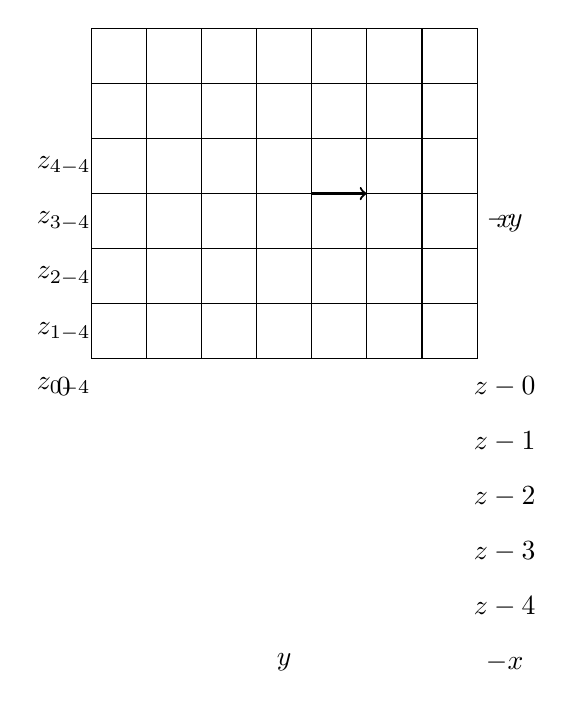
\begin{tikzpicture}[scale=0.7]
    % Define grid lines
    \draw[thin] (0,0) grid (7,6);
    % Left side labels
    \foreach \i in {0,1,...,4}
        \node at (-0.5, \i-0.5) {$z_{\i-4}$};
    \node at (-0.5, -0.5) {0};
    % Right side original label
    \node at (7.5, 2.5) {$x$};
    % Middle arrow
    \draw[->, thick] (4,3) -- (5,3);
    % Right side labels
    \foreach \i in {0,1,...,4}
        \node at (7.5, -\i-0.5) {$z- \i$};
    \node at (7.5, 2.5) {$-y$};
    \node at (7.5, -5.5) {$-x$};
    % Bottom middle label
    \node at (3.5, -5.5) {$y$};
\end{tikzpicture}

\end{document}